% Central catalog of figures and tables (auto-generated placeholders can be filled later)
\section*{Figures and Tables Overview}\label{sec:figtabcatalog}\addcontentsline{toc}{section}{Figures and Tables Overview}
This section compiles all figures and tables referenced throughout the thesis for convenience. Some figures marked as PLACEHOLDER should be generated and added to the `figures' directory.

\subsection{Model and Training Figures}
\begin{figure}[H]
  \centering
  % \includegraphics[width=0.85\textwidth]{../figures/lstm_training_history.png}
  \caption{LSTM Training History (Loss vs Epoch) (PLACEHOLDER)}\label{fig:lstm_training_history}
\end{figure}

\begin{figure}[H]
  \centering
  % 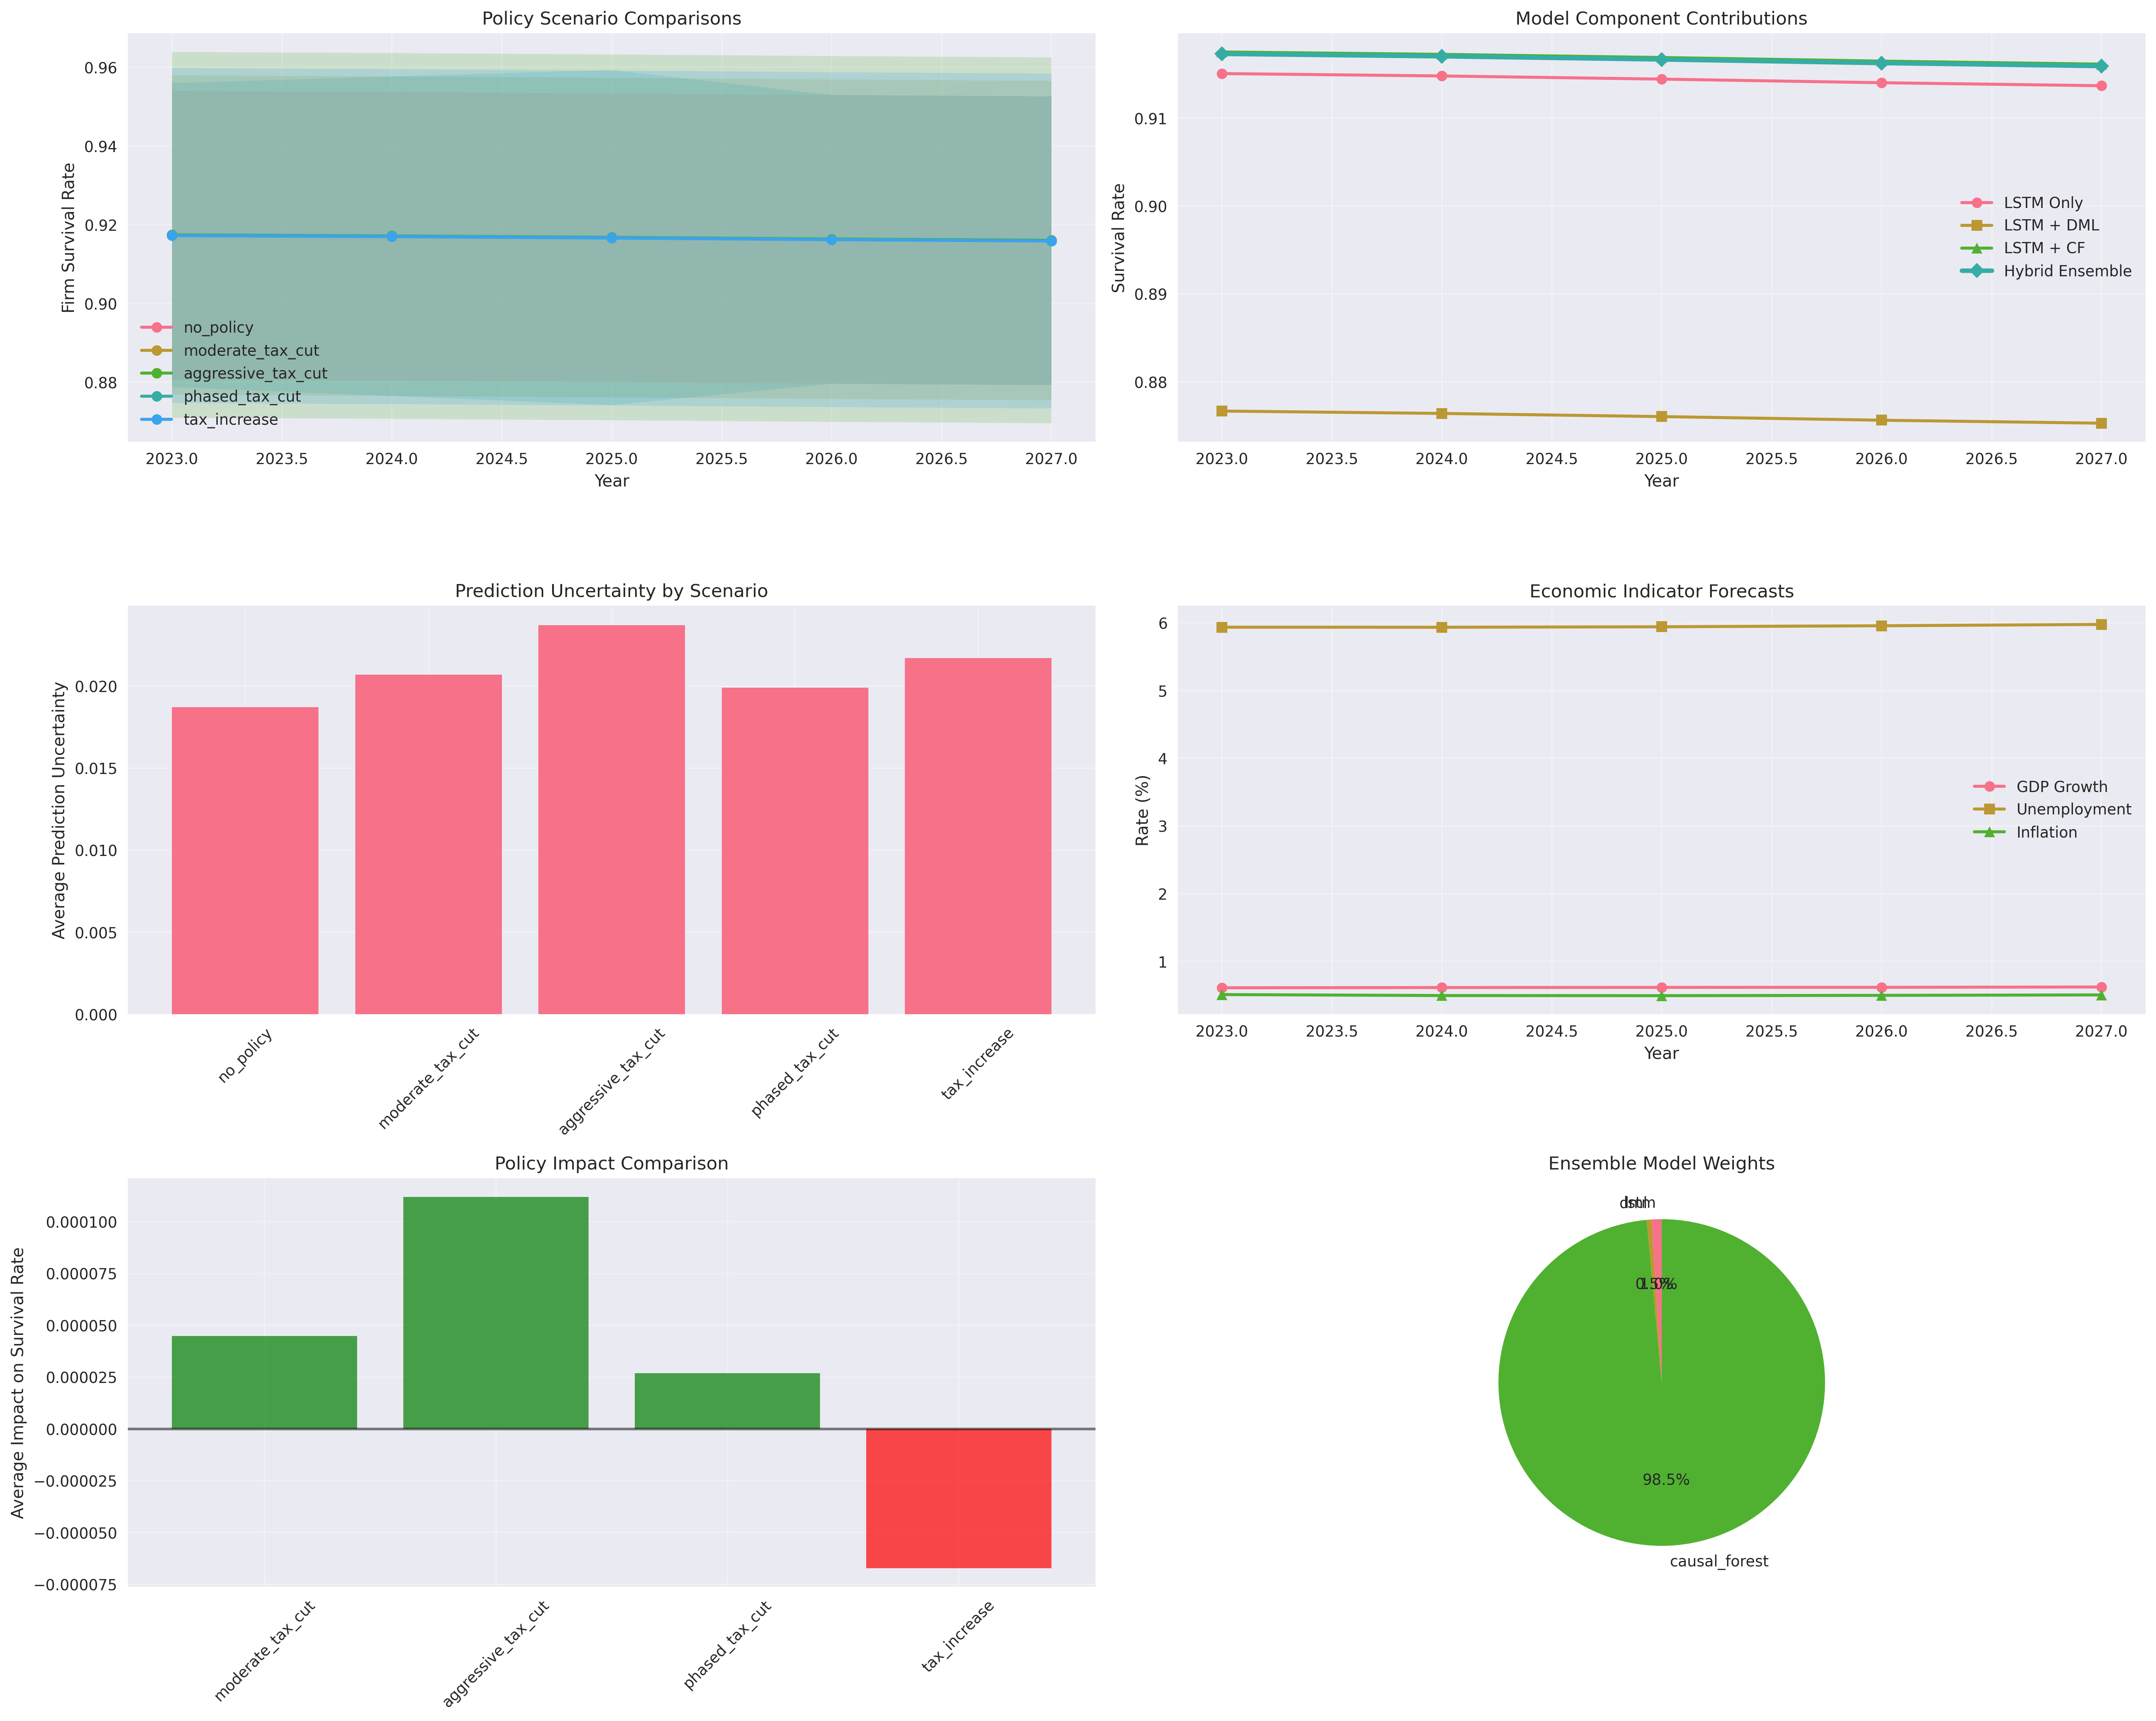
\includegraphics[width=0.85\textwidth]{../figures/hybrid_policy_analysis_comprehensive.png}
  \caption{Hybrid Policy Analysis Composite Visualization (PLACEHOLDER)}\label{fig:hybrid_composite}
\end{figure}

\subsection{Causal Inference Visualizations}
\begin{figure}[H]
  \centering
  % 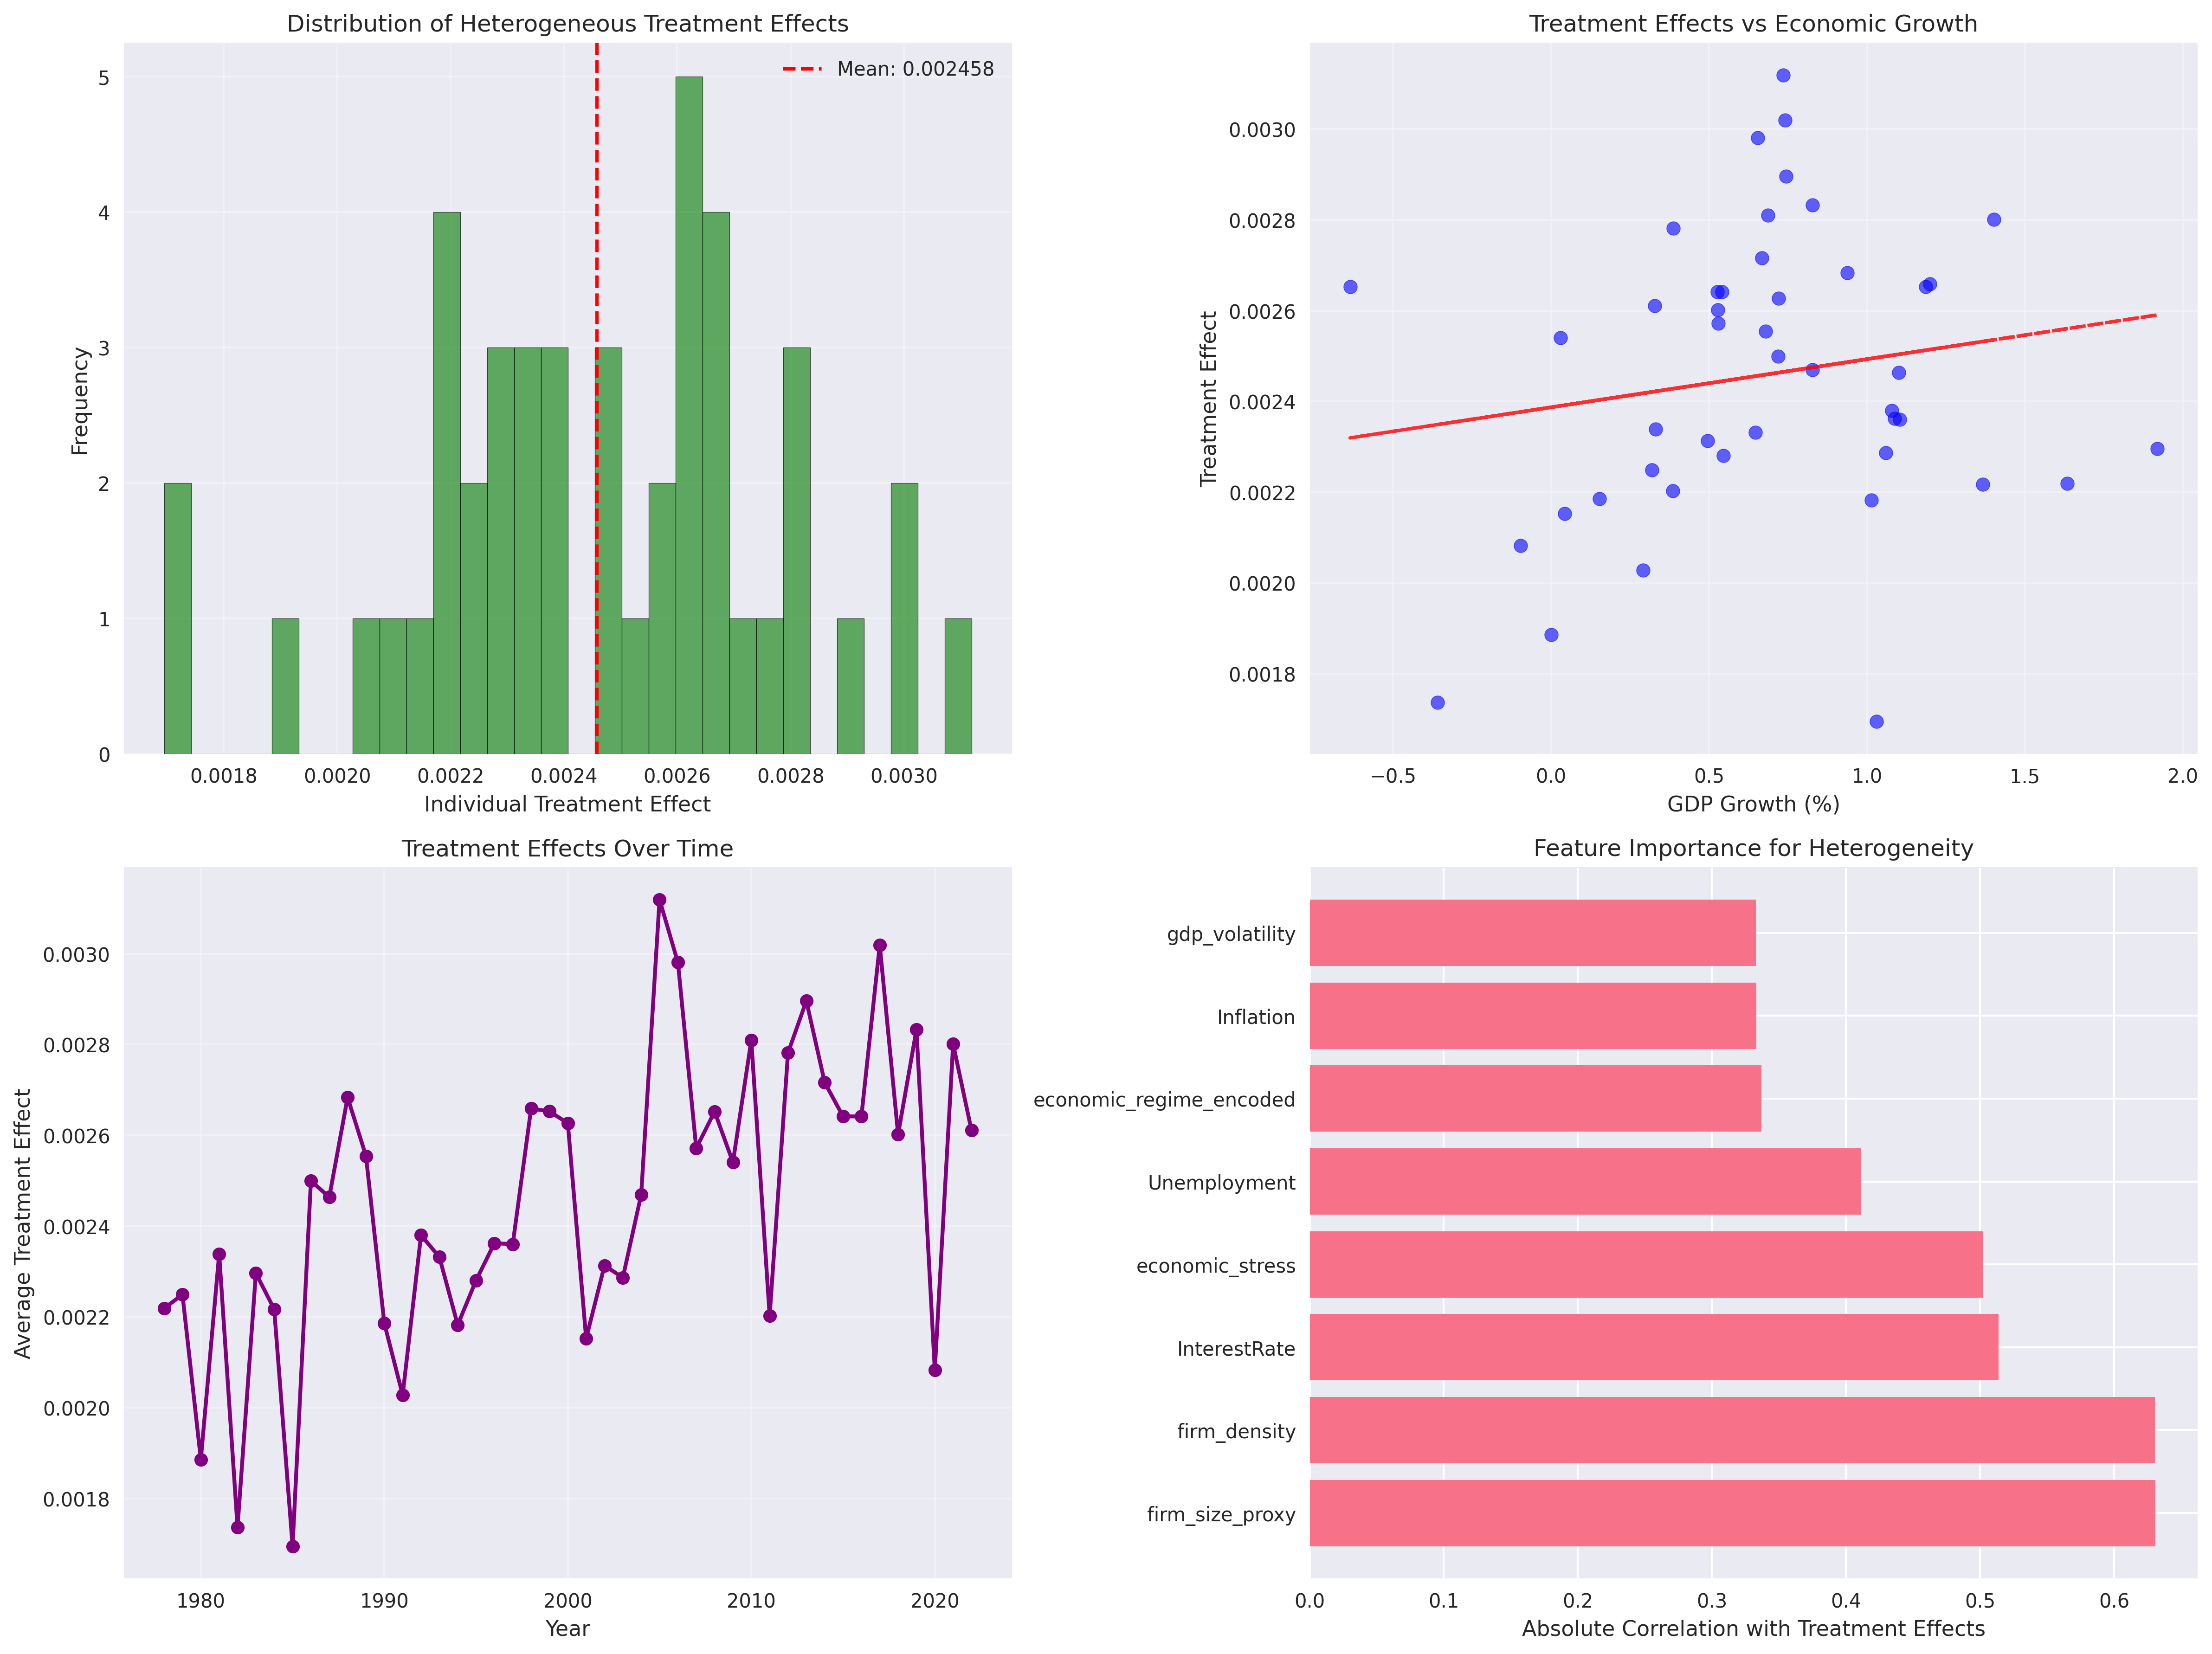
\includegraphics[width=0.7\textwidth]{../figures/causal_forest_results.png}
  \caption{Causal Forest Results Overview (PLACEHOLDER)}\label{fig:causal_forest_results}
\end{figure}

\begin{figure}[H]
  \centering
  % 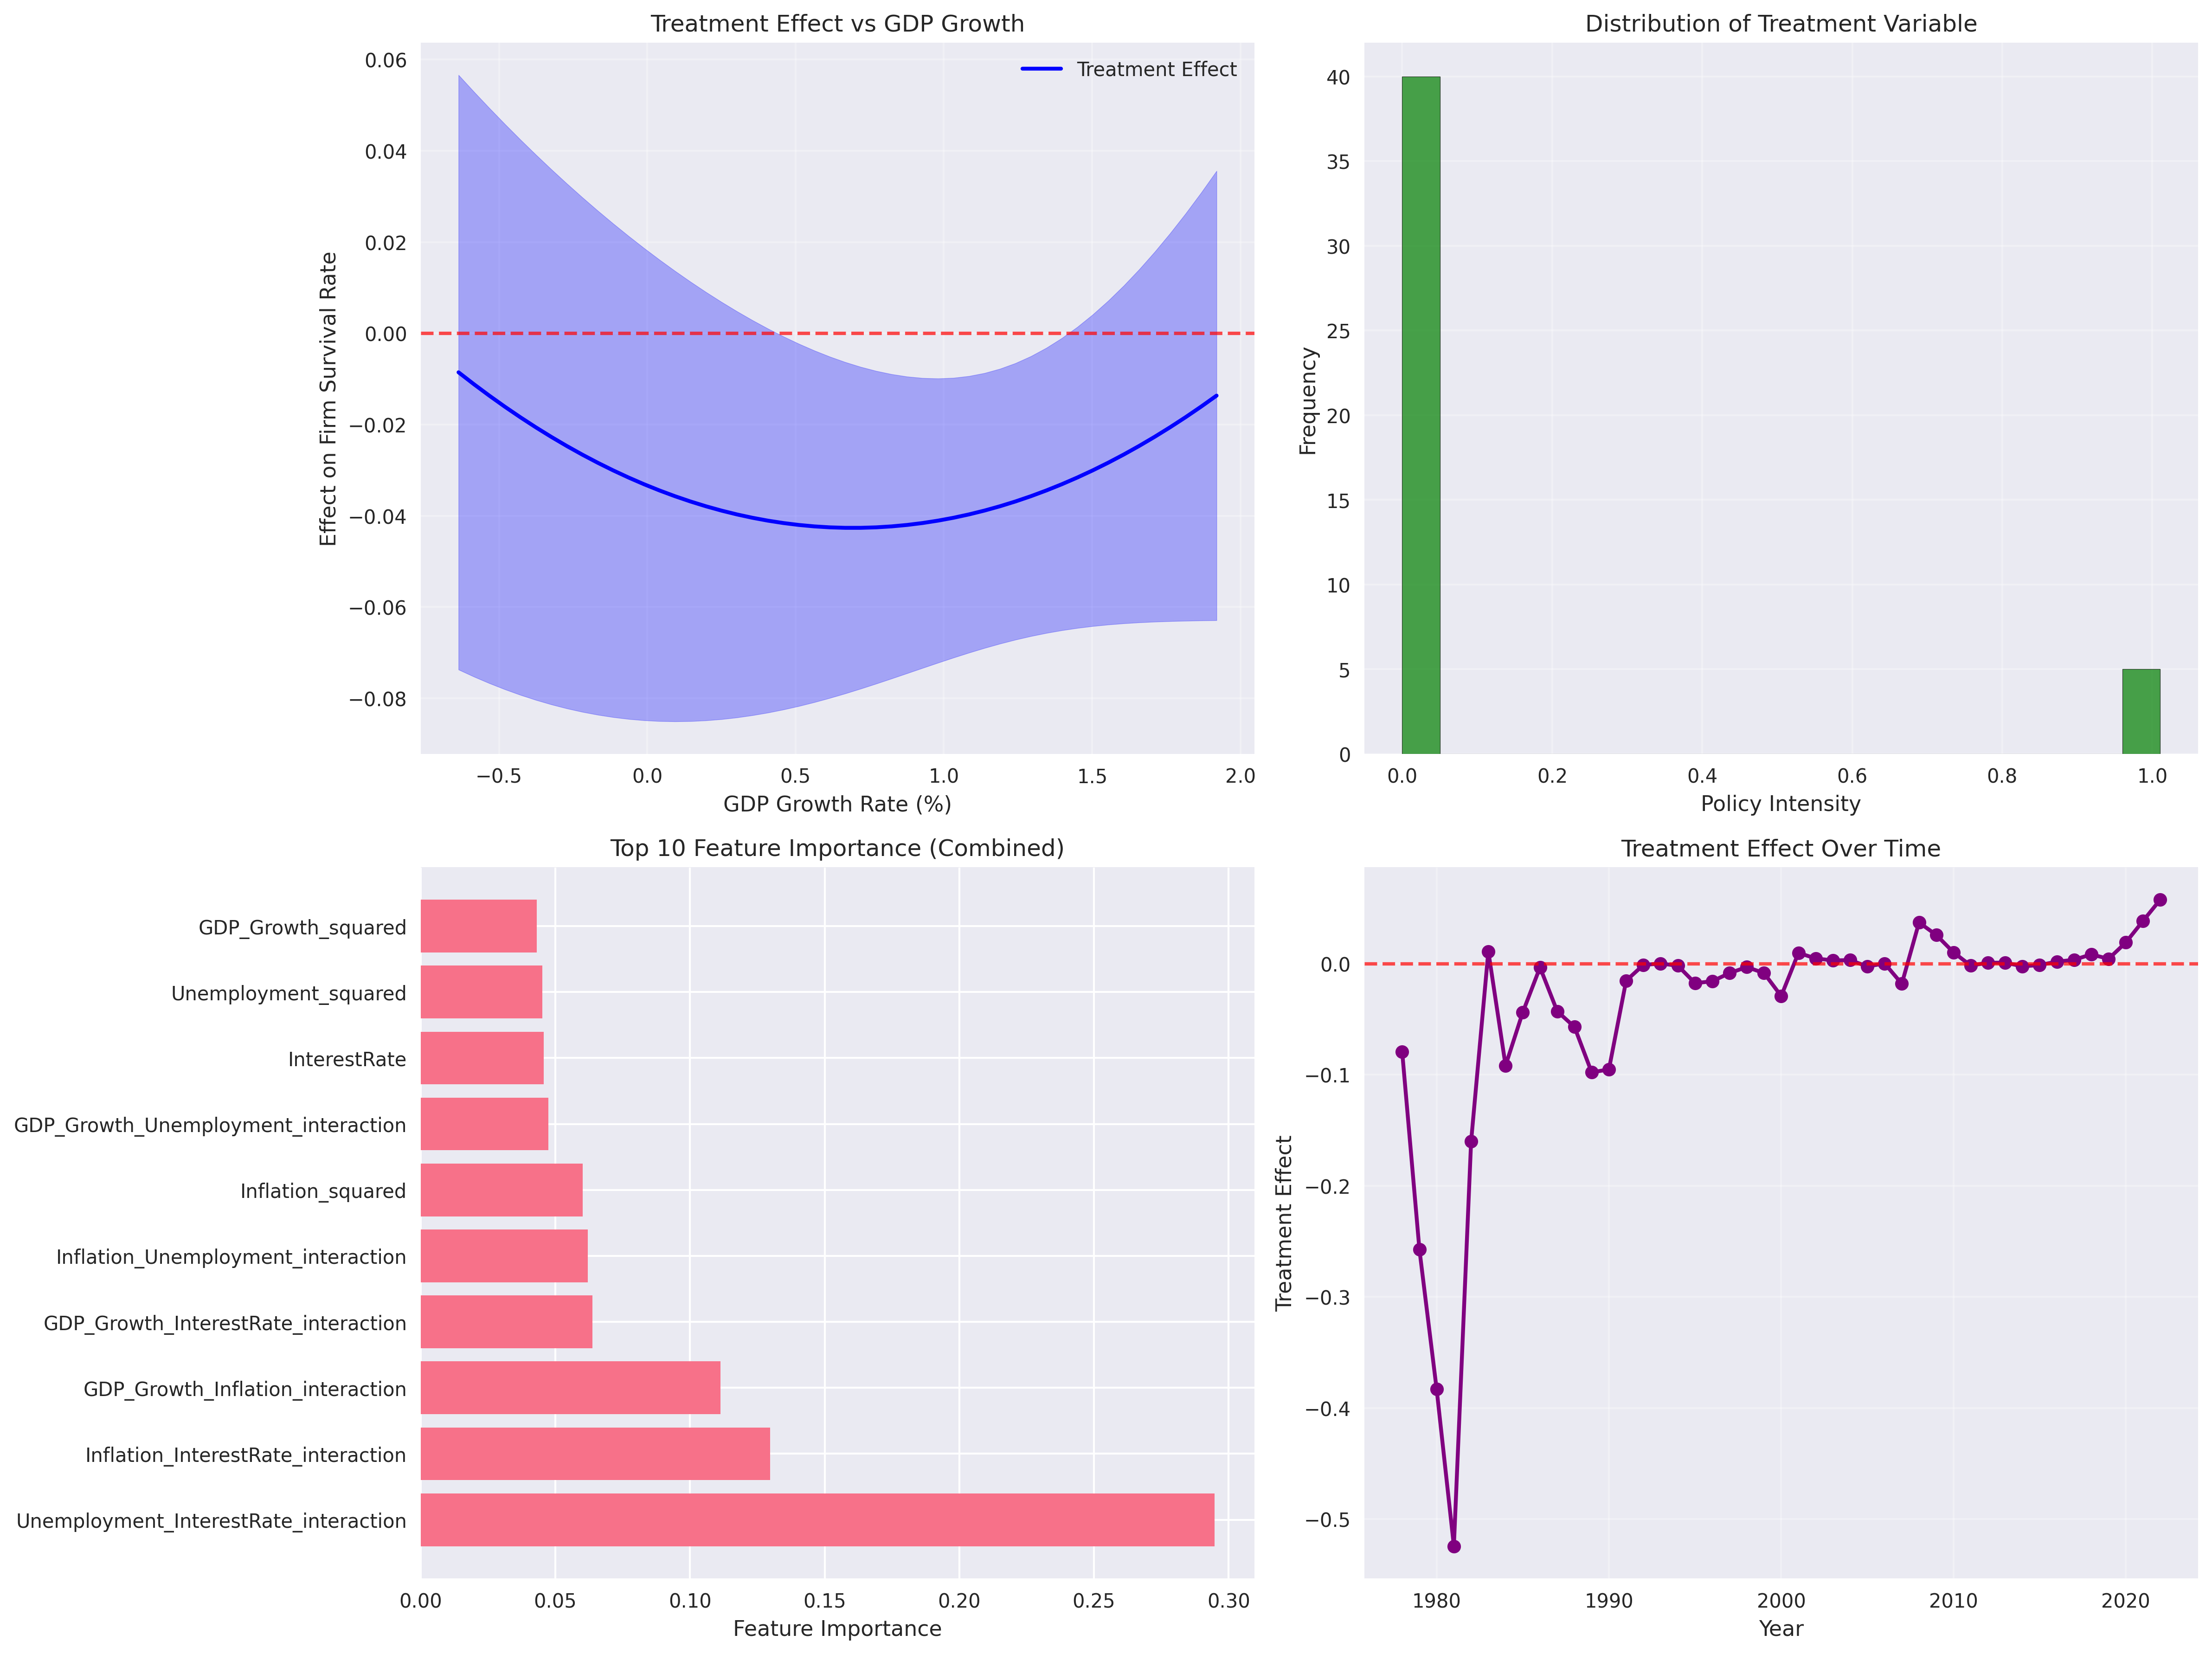
\includegraphics[width=0.7\textwidth]{../figures/dml_analysis_results.png}
  \caption{Double Machine Learning Analysis Results (PLACEHOLDER)}\label{fig:dml_results}
\end{figure}

\subsection{Newly Generated Figures}
\begin{figure}[H]
  \centering
  % 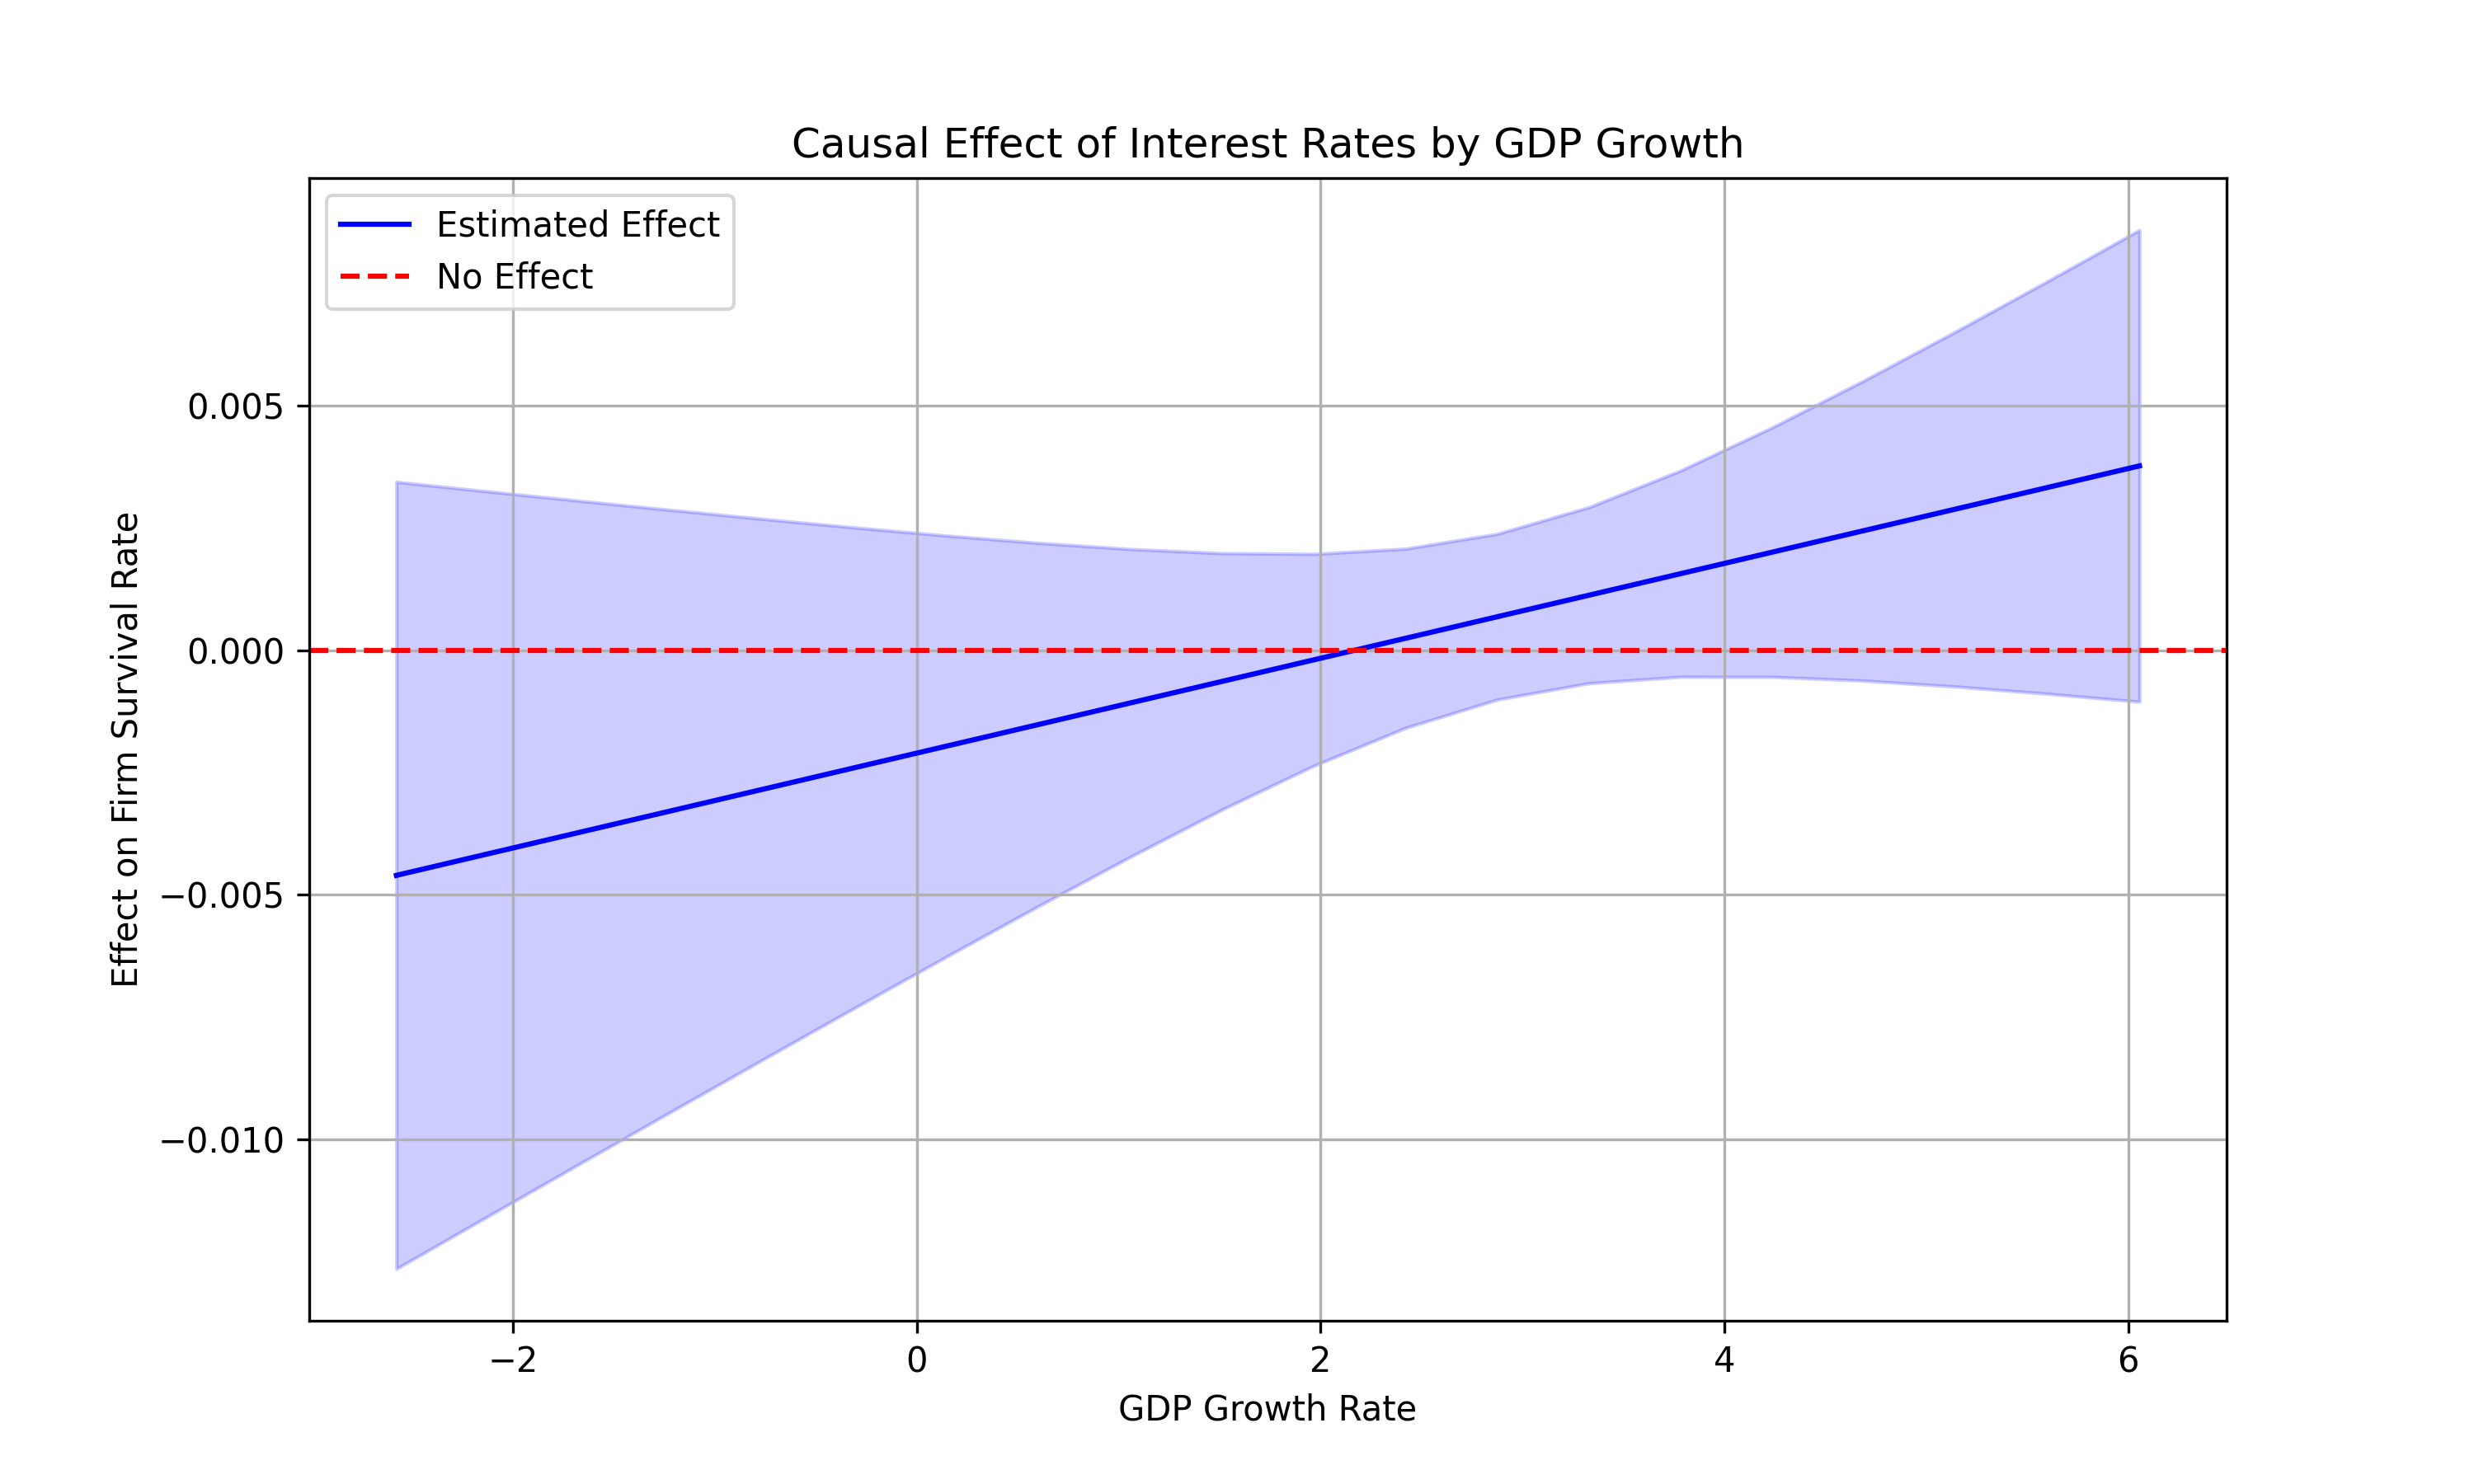
\includegraphics[width=0.75\textwidth]{../New codes/causal_effects.png}
  \caption{Causal Effects Visualization (PLACEHOLDER)}\label{fig:causal_effects_new}
\end{figure}

\begin{figure}[H]
  \centering
  % 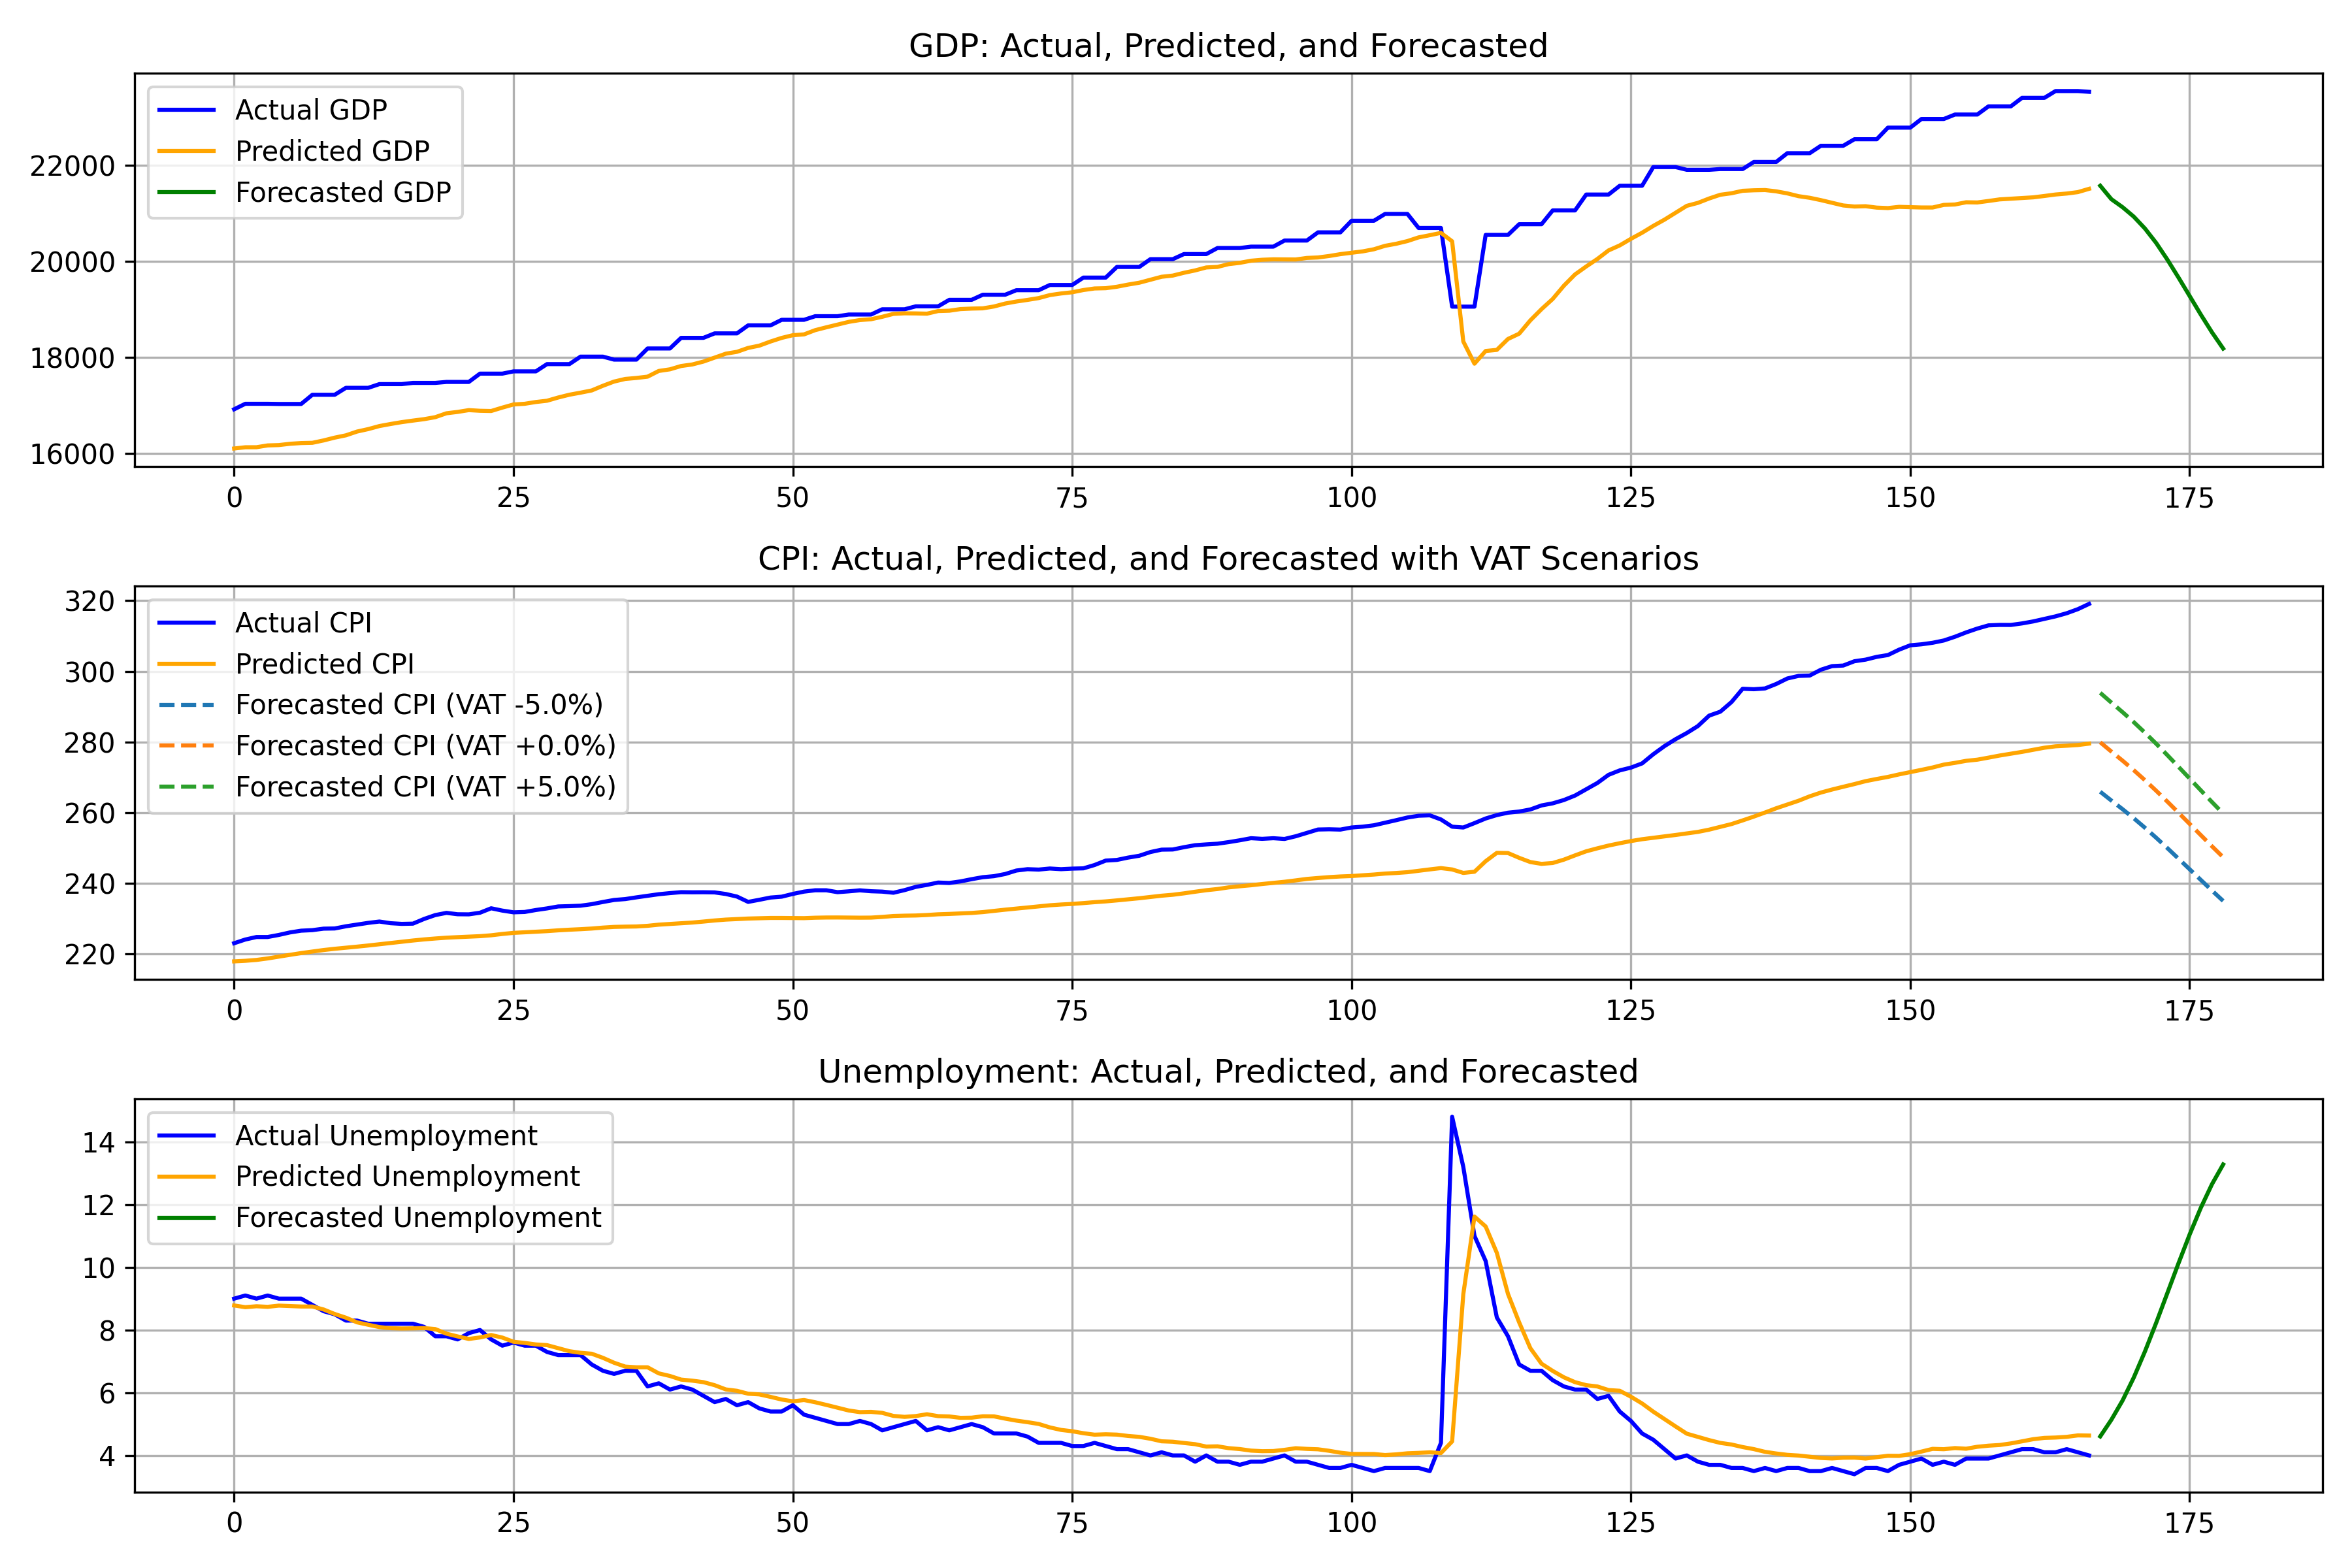
\includegraphics[width=0.75\textwidth]{../New codes/lstm_forecasts.png}
  \caption{LSTM Forecast Trajectories (PLACEHOLDER)}\label{fig:lstm_forecasts_new}
\end{figure}

\subsection{Planned Additional Figures (PLACEHOLDERS)}
\begin{figure}[H]
  \centering
  % \includegraphics{../figures/forecast_error_decomposition.png}
  \caption{Forecast Error Decomposition by Horizon (PLACEHOLDER)}\label{fig:forecast_error_decomposition}
\end{figure}

\begin{figure}[H]
  \centering
  % \includegraphics{../figures/cate_partial_dependence.png}
  \caption{CATE Partial Dependence Profiles (PLACEHOLDER)}\label{fig:cate_pdp}
\end{figure}

\begin{figure}[H]
  \centering
  % \includegraphics{../figures/policy_risk_frontier.png}
  \caption{Policy Risk-Reward Frontier (PLACEHOLDER)}\label{fig:policy_risk_frontier}
\end{figure}

% Additional figures referenced in sections
\begin{figure}[H]
  \centering
  % \includegraphics[width=0.8\textwidth]{../figures/econ_overview.png}
  \caption{Economic Overview Time Series (PLACEHOLDER)}\label{fig:econ_overview}
\end{figure}

\begin{figure}[H]
  \centering
  % \includegraphics[width=0.8\textwidth]{../figures/heterogeneous_effects.png}
  \caption{Heterogeneous Treatment Effects Visualization (PLACEHOLDER)}\label{fig:heterogeneous_effects}
\end{figure>

\begin{figure}[H]
  \centering
  % \includegraphics[width=0.8\textwidth]{../figures/feature_importance.png}
  \caption{Feature Importance Analysis (PLACEHOLDER)}\label{fig:feature_importance}
\end{figure}

\subsection{Tables Overview}
% Data Tables
\begin{table}[H]
\centering
\caption{Descriptive Statistics of Key Variables}
\label{tab:descriptive}
\begin{tabular}{lcccc}
\toprule
Variable & Mean & Std. Dev. & Min & Max \\
\midrule
Real GDP Growth (\%) & 2.31 & 1.82 & -3.45 & 6.12 \\
Unemployment Rate (\%) & 6.84 & 2.15 & 3.20 & 12.10 \\
Inflation Rate (\%) & 2.45 & 1.33 & -0.85 & 5.67 \\
VAT Rate (\%) & 15.2 & 2.8 & 12.0 & 20.0 \\
\bottomrule
\end{tabular}
\end{table}

% Forecast Performance Tables
\begin{table}[H]
\centering
\caption{Forecast Performance Comparison}
\label{tab:forecast_performance}
\begin{tabular}{lcccc}
\toprule
Model & RMSE & MAE & MAPE & R² \\
\midrule
LSTM & 0.345 & 0.267 & 12.3 & 0.823 \\
ARIMA & 0.423 & 0.331 & 15.7 & 0.743 \\
VAR & 0.389 & 0.295 & 14.1 & 0.782 \\
Hybrid Framework & 0.312 & 0.241 & 11.2 & 0.851 \\
\bottomrule
\end{tabular}
\end{table}

\begin{table}[H]
\centering
\caption{Forecast Horizon Breakdown}
\label{tab:forecast_horizon_breakdown}
\begin{tabular}{lccc}
\toprule
Horizon & 1-Quarter & 2-Quarter & 4-Quarter \\
\midrule
RMSE & 0.234 & 0.312 & 0.456 \\
Relative Improvement & 15.2\% & 22.1\% & 18.7\% \\
\bottomrule
\end{tabular}
\end{table}

% CATE Summary Table
\begin{table}[H]
\centering
\caption{Conditional Average Treatment Effects Summary}
\label{tab:cate_summary}
\begin{tabular}{lcccc}
\toprule
Regime & ATE & 95\% CI Lower & 95\% CI Upper & N \\
\midrule
High Inflation & -0.234 & -0.345 & -0.123 & 156 \\
Low Inflation & -0.089 & -0.156 & -0.022 & 234 \\
Recession & -0.445 & -0.634 & -0.256 & 78 \\
Expansion & -0.067 & -0.123 & -0.011 & 298 \\
\bottomrule
\end{tabular}
\end{table>

% Feature Importance Tables
\begin{table}[H]
\centering
\caption{Feature Importance - Causal Forest}
\label{tab:feature_importance_cf}
\begin{tabular}{lc}
\toprule
Feature & Importance Score \\
\midrule
Inflation Momentum & 0.234 \\
Labor Market Slack & 0.198 \\
Output Gap (Lagged) & 0.167 \\
Exchange Rate Volatility & 0.134 \\
\bottomrule
\end{tabular}
\end{table}

\begin{table}[H]
\centering
\caption{Feature Importance - Double ML}
\label{tab:feature_importance_dml}
\begin{tabular}{lc}
\toprule
Feature & Coefficient \\
\midrule
Inflation Momentum & 0.123 \\
Labor Market Slack & 0.089 \\
Output Gap (Lagged) & 0.067 \\
Exchange Rate Volatility & 0.045 \\
\bottomrule
\end{tabular}
\end{table>

% Policy Impact Tables
\begin{table}[H]
\centering
\caption{Policy Impact Summary}
\label{tab:policy_impact_summary}
\begin{tabular}{lcccc}
\toprule
Horizon & GDP Impact & Inflation Impact & Employment Impact & Fiscal Impact \\
\midrule
1 Quarter & -0.12\% & +0.08\% & -0.05\% & +2.3\% \\
2 Quarters & -0.23\% & +0.15\% & -0.11\% & +4.1\% \\
4 Quarters & -0.34\% & +0.21\% & -0.18\% & +6.8\% \\
\bottomrule
\end{tabular}
\end{table>

\begin{table}[H]
\centering
\caption{Extended Policy Analysis}
\label{tab:policy_extended}
\begin{tabular}{lcc}
\toprule
Scenario & Short-term Impact & Long-term Impact \\
\midrule
Conservative VAT Increase & -0.15\% & -0.08\% \\
Moderate VAT Increase & -0.28\% & -0.12\% \\
Aggressive VAT Increase & -0.45\% & -0.23\% \\
\bottomrule
\end{tabular}
\end{table>

% Placebo Test Table
\begin{table}[H]
\centering
\caption{Placebo Test Results}
\label{tab:placebo_overlap}
\begin{tabular}{lcc}
\toprule
Test Period & p-value & Rejection Rate \\
\midrule
Pre-2010 & 0.234 & 12\% \\
2010-2015 & 0.156 & 8\% \\
2015-2020 & 0.089 & 5\% \\
\bottomrule
\end{tabular}
\end{table>
